\section{Braintree}
\label{sec:braintree}
Braintree is a full-stack payments platform that makes it easy to accept payments in your app or website. Our service replaces the traditional model of sourcing a payment gateway and merchant account from different providers. From one touch payments to mobile SDKs and foreign currency acceptance, we provide everything you need to start accepting payments today.
\newline
All kinds of organizations use Braintree to accept payments in mobile apps and websites. From startups in garages, to not-for-profits, to some of the largest online retailers, we have more experience working with new business models than any other payments provider. However, due to legal and regulatory compliance reasons, Braintree isn't able to work with some business types. How to use Braintree as a payment system?
Braintree's  consists of complementary client and server SDKs:
\begin{itemize}
  \item The client SDK enables you to collect payment method (e.g. credit card, PayPal) details;
  \item The server SDKs manage all requests to the Braintree gateway
\end{itemize}
Before we get started, there are two key concepts to introduce - the client token and the payment method nonce.
\newline
SDK Braintree offer various options to the programmer to integrate the payment service.
\begin{figure}[htb]
  \centering
  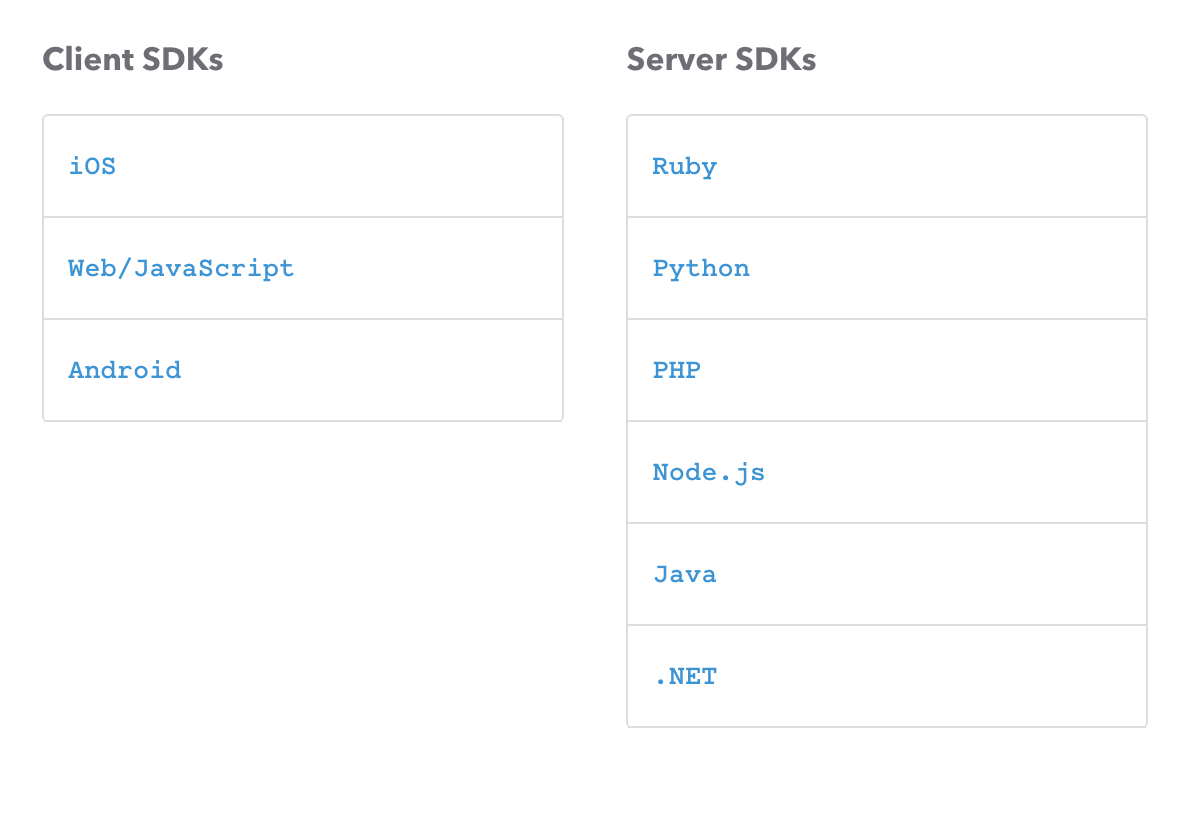
\includegraphics[width=1.0\linewidth]{images/chapter3/braintree-sdk.png}\hfill
  \caption[Braintree SDK]{Braintree SDK}
\label{fig:braintree_sdk}
\end{figure}
\subsection{Client Token}
A client token is a signed data blob that includes configuration and authorization information required by the Braintree Client SDK. These should not be reused; a new client token should be generated for each customer request that's sent to Braintree. For security, Braintree server revoke client tokens if they are reused excessively within a short time period.
The server is responsible for generating the client token, which contains all of the necessary configuration information to set up the client SDKs. When your server provides a client token to your client, it authenticates the application to communicate directly to Braintree.
The client is responsible for obtaining the client token and initializing the client SDK. If this succeeds, the client will generate a \emph{payment\_method\_nonce}.
\subsection{Payment Method Nonce}
The payment method nonce is a string returned by the client SDK to represent a payment method. This string is a reference to the customer payment method details that were provided in your payment form and should be sent to your server where it can be used with the server SDKs to create a new transaction request.
\begin{figure}[htb]
  \centering
  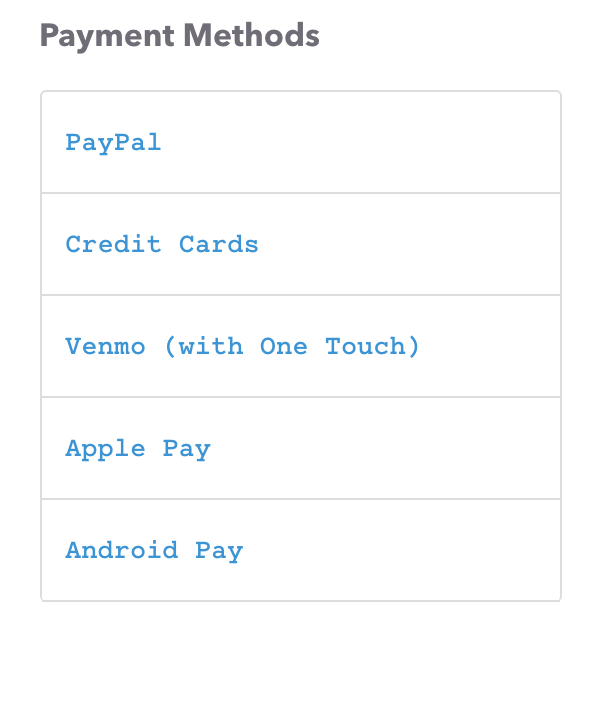
\includegraphics[width=0.4\linewidth]{images/chapter3/braintree-payment-method.png}\hfill
  \caption[Braintree payment method]{Braintree payment method}
  \label{fig:braintree_payment_method}
\end{figure}
Payment method nonces expire after 24 hours.
The server integration doesn't need to know the payment method type (e.g. credit card, PayPal account, Bitcoin) that is represented in the nonce. This means that your first v.zero integration should continue to work with few or no code changes when new payment method types are introduced.
\subsection{How it work}
\begin{figure}[htb]
  \centering
  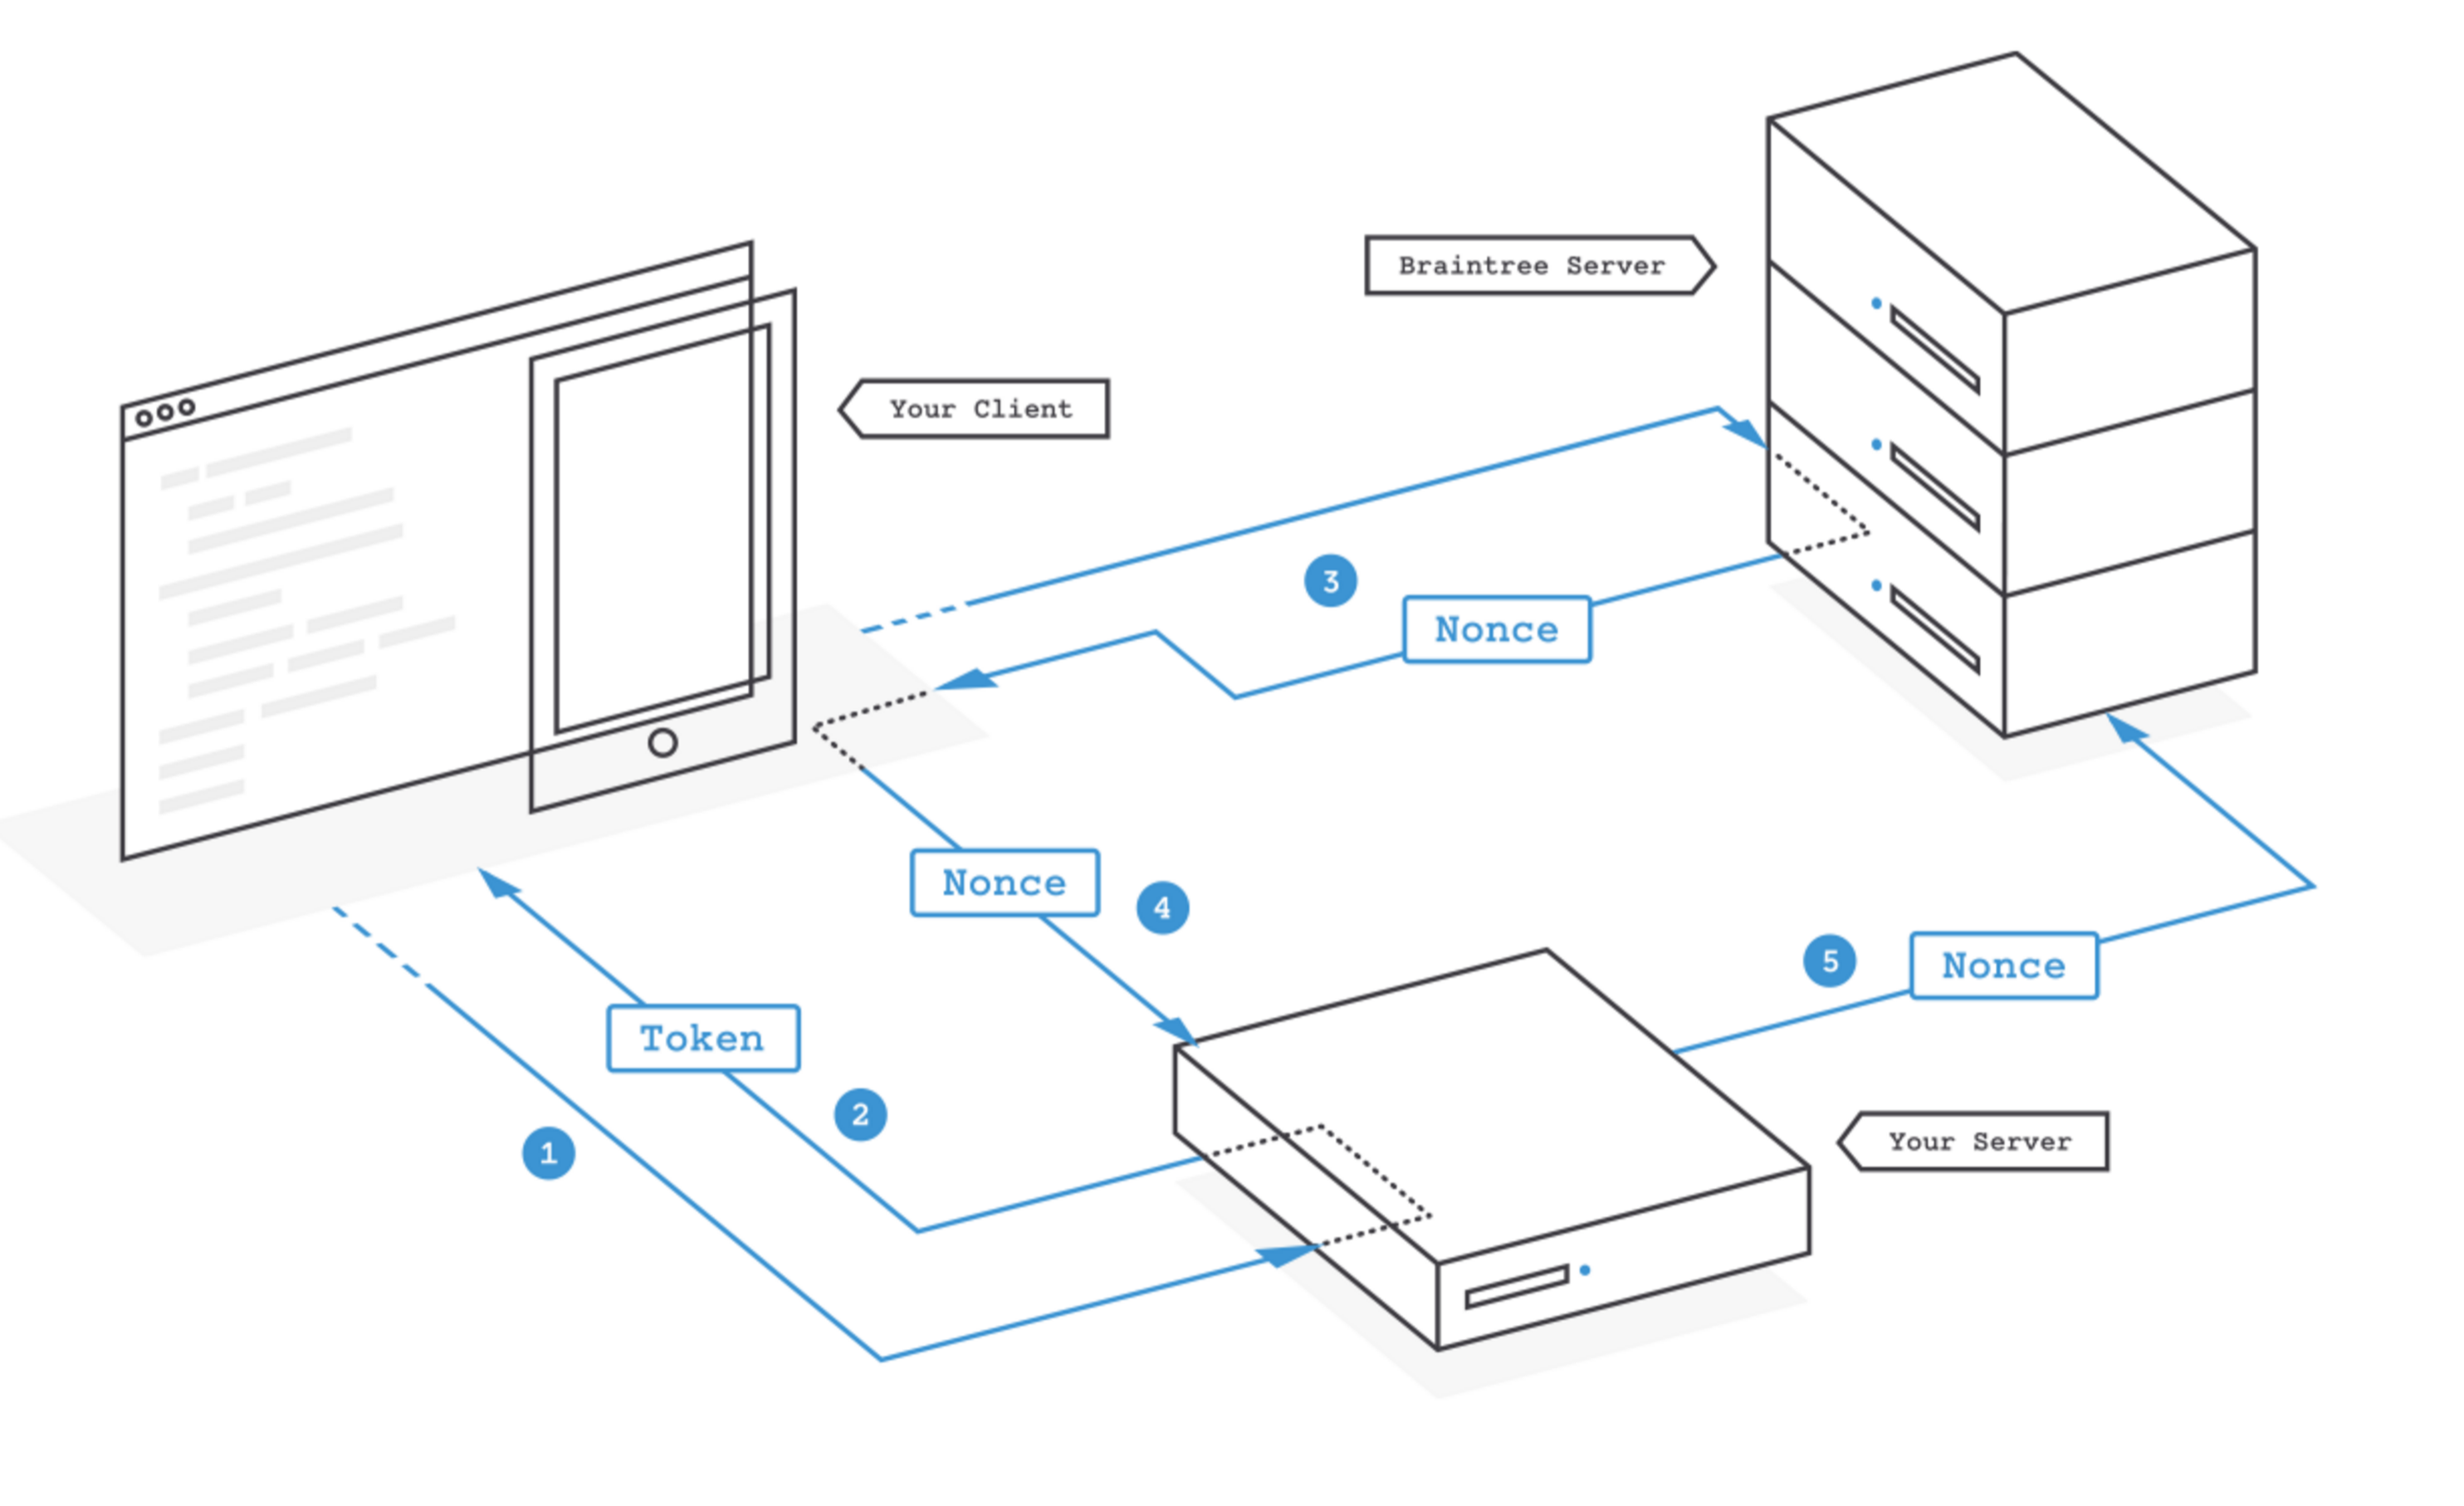
\includegraphics[width=1.0\linewidth]{images/chapter3/braintree-comunicaiton.png}\hfill
  \caption[Interaction client-braintree]{Comunication between client and server braintree step by step}
  \label{fig:braintree_server_comunication}
\end{figure}
\begin{enumerate}
  \item App or web front-end requests a client token from your server in order to initialize the client SDK;
  \item Server generates and sends a client token back to your client with the server SDK;
  \item Once the client SDK is initialized and the customer has submitted payment information, the SDK communicates that information to Braintree, which returns a payment method nonce;
  \item Then send the payment nonce to your server;
  \item Server code receives the payment method nonce from your client and then uses the server SDK to create a transaction or perform other Braintree functions.
\end{enumerate}
The easiest way to use braintree is through Drop-in UI. This type of configuration is certainly the simplest but allows the programmer to customize the input form for entering your payment information. The interface Drop-in looks like this as follows:
\begin{figure}[htb]
  \centering
  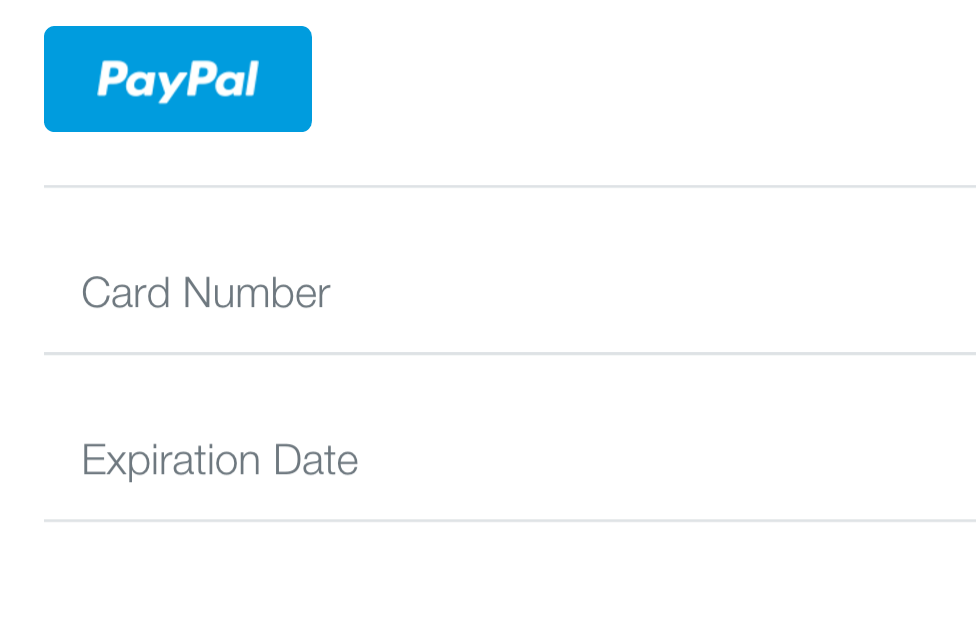
\includegraphics[width=0.6\linewidth]{images/chapter3/drop-in.png}\hfill
  \caption[Drop-in UI]{ Drop-in UI}
  \label{fig:drop_in_ui}
\end{figure}
To create and maintain this form to the client-side you must import the scrip \emph{brantree.js} and organize form so as follows:
\begin{lstlisting}[language=html]
<form id="checkout" method="post" action="/checkout">
  <div id="payment-form"></div>
  <input type="submit" value="Pay $10">
</form>

<script src="https://js.braintreegateway.com/v2/braintree.js"></script>
<script>
// We generated a client token for you so you can test out this code
// immediately. In a production-ready integration, you will need to
// generate a client token on your server.
var clientToken = client_token;

braintree.setup(clientToken, "dropin", {
  container: "payment-form"
});
</script>
\end{lstlisting}
To start up, braintree.js needs a client-token generated by your Braintree server SDK. The client-token is unique.
\newline
There are a number of ways to get your client token into JavaScript so you can set up Braintree. Many people choose to interpolate the client token into the HTML/JavaScript itself; alternatively, you could load the client token from an AJAX call to your exposed client token URL on your server.
Once you've finished this setup. Now we are ready to make payments.
\newline
A Braintree client-side integration sends payment information – like a credit card or a PayPal authorization – to Braintree in exchange for a payment method nonce, a one time use value that represents that payment method.
On your server, use a payment method nonce with a Braintree server SDK to charge a card or update a customers' payment methods.
\newline
By default, \emph{braintree.js} will add a hidden input named \emph{payment\_method\_nonce} to your form. When your user submits the form, if you have not subscribed to the \emph{onPaymentMethodReceived} callback, your form will be submitted with this value.
\newline
Braintree provides a sandbox for developers account, credit cards test for testing your application.
That said, we would like to use a form that is customizable to the way we would like to stylize the payment form without using the default. To do this simply specify additional parameters to the client side. How does this see in Chapter 5.